\appendix

\begin{frame}[noframenumbering, plain]{}
    Backup slides
\end{frame}

% XXX write those
\begin{frame}{MR signal derivation}

\end{frame}

\begin{frame}{Fourier Transform and MRI}

\end{frame}

\begin{frame}{More details on GRAPPA}

\end{frame}

\begin{frame}{Sparsity}

\end{frame}

\begin{frame}{Basis Pursuit}

\end{frame}

\begin{frame}{Sensitivity Maps}

\end{frame}

\begin{frame}{Noise model for MRI}

\end{frame}

\begin{frame}{Proximity operator}

\end{frame}

\begin{frame}{Convolutions}

\end{frame}

\begin{frame}{CNN}
    Convolutional Neural Network~(CNN): chain of Convolution + Nonlinearity.
\end{frame}

\begin{frame}{U-net}
    \begin{figure}
        \centering
        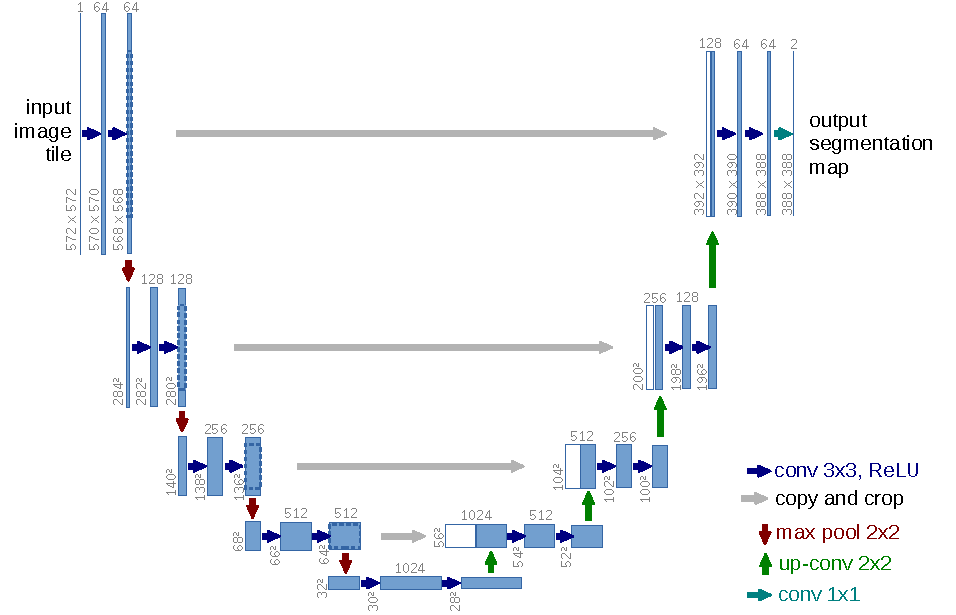
\includegraphics[height=0.6\textheight]{Figures/add_slides/unet_hires.pdf}
        \caption{Illustration from the original paper.\footfullcite{ronneberger2015u}}
    \end{figure}
\end{frame}

\begin{frame}{MWCNN}
    \begin{figure}
        \centering
        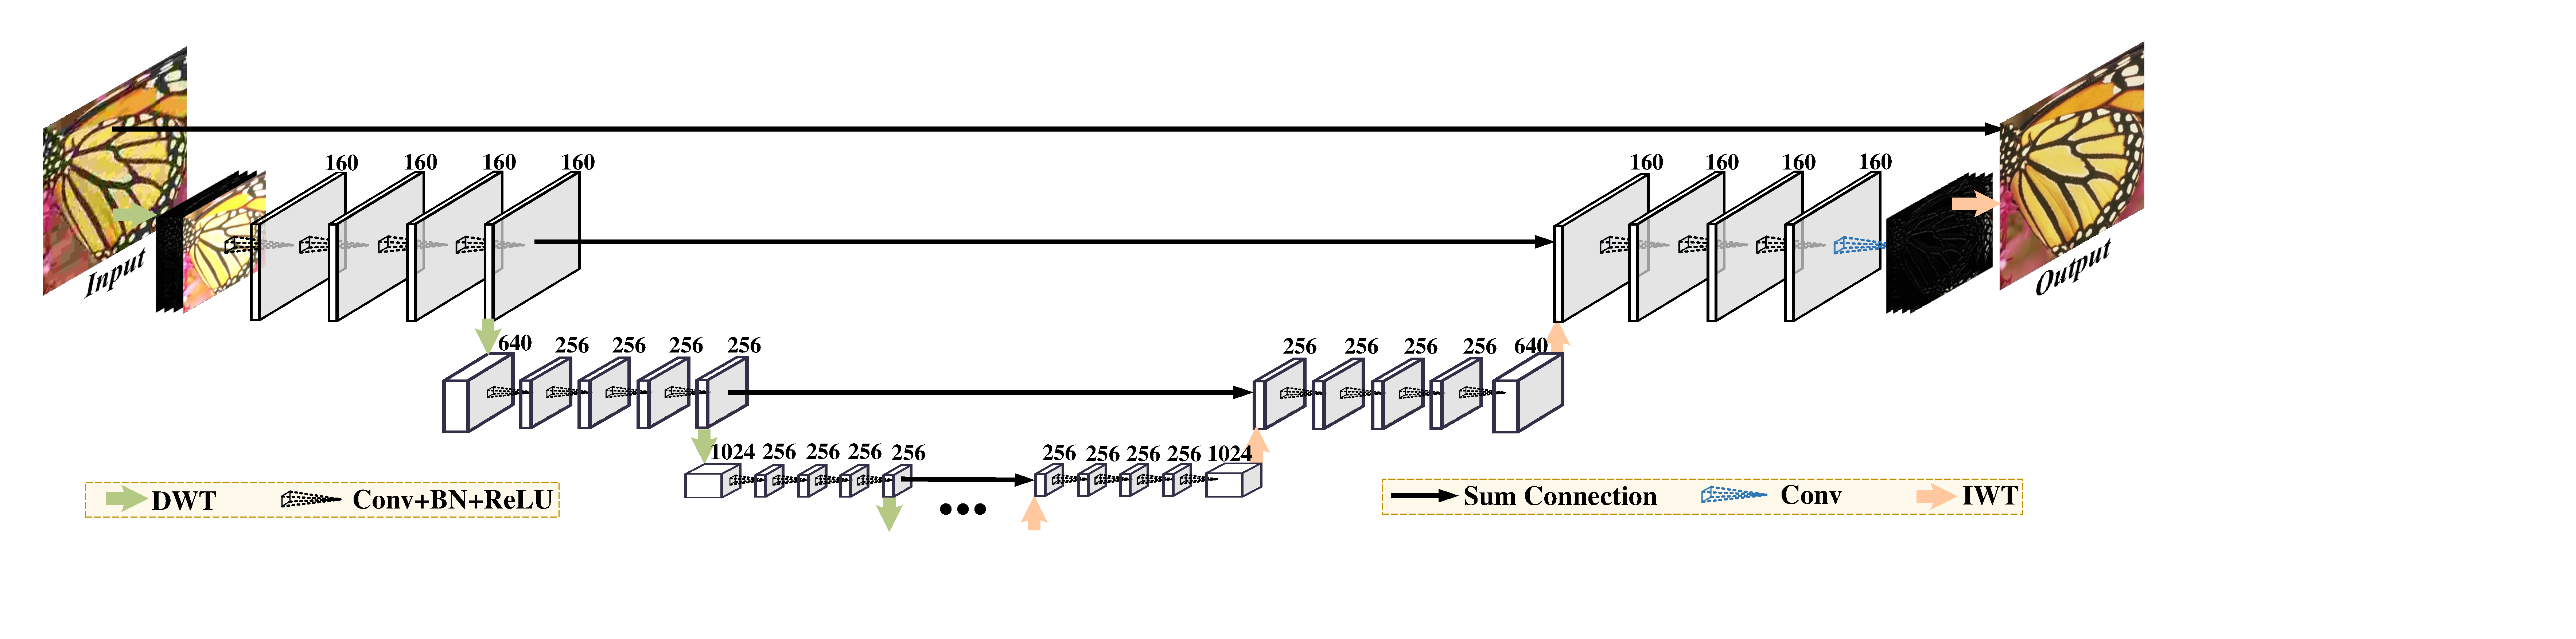
\includegraphics[width=\textwidth]{Figures/add_slides/mwcnn.pdf}
        \caption{Illustration from the original paper.\footfullcite{Liu2018}}
    \end{figure}
\end{frame}

\begin{frame}{fastMRI dataset}

\end{frame}

\begin{frame}{fastMRI challenge}

\end{frame}

\begin{frame}{autoMAP}

\end{frame}

\begin{frame}{XPDNet - ct'ed}
    % only writing the algos
\end{frame}

\begin{frame}{PDNet \& Recurent Inference Machines}

\end{frame}

\begin{frame}{NC-PDNet - ct'ed}
    % only writing the algos
\end{frame}

\begin{frame}{Density Compensation}

\end{frame}

\begin{frame}{Image quality metrics}

\end{frame}

\begin{frame}{quasi-Newton methods}

\end{frame}

\begin{frame}{OPA - 1}

\end{frame}

\begin{frame}{OPA - 2}
    \begin{center}
        \scalebox{.5}{
    \begin{algorithm}[H]
        \SetAlgoRefName{LBFGS}
        \DontPrintSemicolon
        \caption{(Limited memory) BFGS method with OPA.}
        \label{alg:LBFGS}
        \KwIn{ initial guess $(\zb_0, \Bb_0^{-1})$, where $\Bb_0^{-1}$ is symmetric and positive definite, tolerance $\epsilon>0$, frequency of additional updates $M\in\mathbb{N}$, memory limit $L\in\mathbb{N}\cup\{\infty\}$, $(t_n)$ a null sequence of positive numbers with $\sum_n t_n<\infty$	}
        Let $F := \nabla_\zb g_{\theta}$\\
        \For{ $n=0,1,2,\ldots$ }
        {
            \lIf{$\norm{F(\zb_n)}\leq\epsilon$ }{let $\zb^\star:=\zb_n$ and let $\Bb:=\Bb_n$; STOP}
            Let $\hat \Bb_n^{-1}:=\Bb_n^{-1}$\\
            \If{$(n\operatorname{mod} M)=0$}{let $\eb_n:=t_n \Bb_n^{-1} \frac{\partial g_{\theta}}{\partial \theta}\Bigr|_{\zb_n}$,
                $\hat \yb_n:=F(\zb_n+\eb_n)-F(\zb_n)$ and $\hat \rb_n:=(\eb_n)^\top \hat \yb_n$\\
            \If{$\hat \rb_n>0$}{let $\hat \ab_n:=\eb_n - \Bb_n^{-1} \hat \yb_n$ and let
            \begin{equation*}
                \hat \Bb_n^{-1} := \Bb_n^{-1} + \frac{\hat \ab_n (\eb_n)^\top + \eb_n (\hat \ab_n)^\top}{\hat \rb_n} -
                \frac{(\hat \ab_n)^\top \hat \yb_n}{(\hat \rb_n)^2} \eb_n (\eb_n)^\top
            \end{equation*}
            }
        }
            Let $\Bb_n^{-1}:=\hat \Bb_n^{-1}$\\
            \lIf{$n\geq L$}{remove update $n-L$ from $\Bb_n^{-1}$}
            Let $p_n := -\Bb_n^{-1} F(\zb_n)$\\
            Obtain $\alpha_n$ via line-search and let $\sb_n := \alpha_n p_n$\\
            Let $\zb_{n+1}:=\zb_n+\sb_n$, $\yb_n:=F(\zb_{n+1})-F(\zb_n)$ and $\rb_n:=(\sb_n)^\top \yb_n$\\
            \uIf{$\rb_n>0$}{let $\ab_n:=\sb_n-\Bb_n^{-1} \yb_n$ and let
            \begin{equation*}
                \Bb_{n+1}^{-1} := \Bb_n^{-1} + \frac{\ab_n (\sb_n)^\top + \sb_n (\ab_n)^\top}{\rb_n} -
                \frac{(\ab_n)^\top \yb_n}{(\rb_n)^2} \sb_n (\sb_n)^\top
            \end{equation*}
            }
            \lElse{let $\Bb_{n+1}^{-1}:=\Bb_n^{-1}$}
            \lIf{$n\geq L$}{remove update $n-L$ from $\Bb_{n+1}^{-1}$}
        }
        \KwOut{$\zb^\star$, $\Bb$}
    \end{algorithm}
    }
    \end{center}
\end{frame}

\begin{frame}{Jacobian-Free}

\end{frame}